% \documentclass[12pt,a4paper]{book}
\documentclass[12pt]{extreport}
\usepackage[utf8]{inputenc} 
\usepackage{amsmath} 
\usepackage{amsfonts} 
\usepackage{amssymb} 
\usepackage{graphicx}
\usepackage{geometry}
 \geometry{
 a4paper,
 total={170mm,257mm},
 left=20mm,
 right=20mm,
 bottom=20mm,
 top=40mm,
 }
\usepackage{draftwatermark} 
\usepackage{textcomp} 
\date{07-09-2018} 
\author{Philip Martin Taylor} 
\title{TaylorWorld Leaflet} 
\begin{document} 
\begin{center} 
\textbf{Welcome to TaylorWorld\texttrademark} 
\end{center} 
\begin{figure}[h]
  \centering
  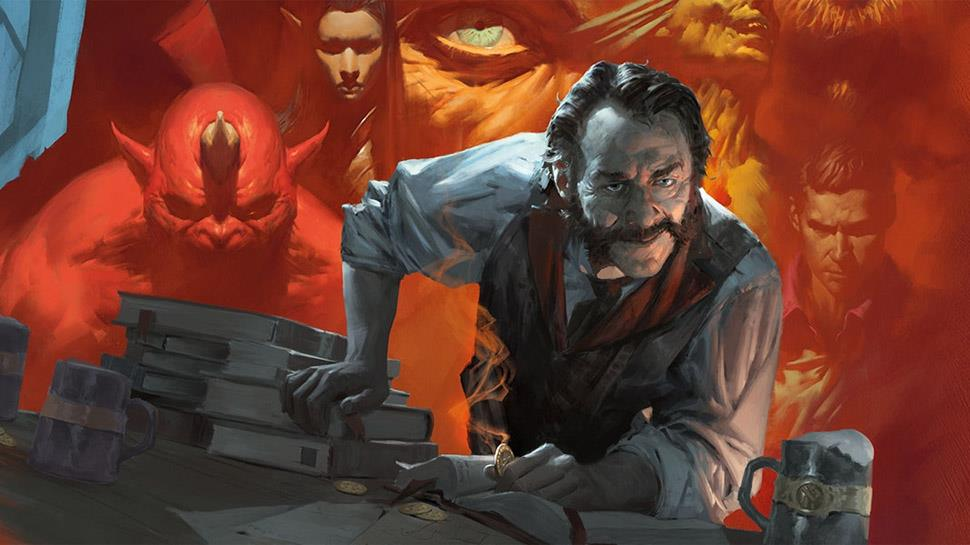
\includegraphics[scale=0.15]{alchemist.jpg}
  % \caption{Lego Wizard}
\end{figure}
\begin{flushleft} We are experts in the Table Top RPG's, Dungeons and Dragons, Pathfinder and Starfinder. Our website is https://odoo.taylorworld.one and our contact email is ptaylor@taylorworld.one. 
\end{flushleft} 
\begin{flushleft}
  If you see this leaflet and your interested in exploring these Table Top Games, either email us, show your interest in the Bailiffs Tap in Banbury, Oxfordshire and ask for Dan, or leave a message on our Facebook page https://www.facebook.com/brobostigon/ . 
\end{flushleft} 
\begin{flushleft}
 We will be hosting games and information sessions at the Bailiffs Tap in Banbury, Oxfordshire, which we will publish on our Facebook Page, where you can get reacquainted with the Table Top RPG's you love and remember, as well as for people newly interested in table top rpg's, to start their learning experience with us. We will be doing taster sessions as well, of the released versions of Dungeons and Dragons, Pathfinder and Starfinder. With Dungeons and Dragons, we specifically specialise in the First Edition of Advanced Dungeons and Dragons.
\end{flushleft} 
\begin{flushleft}
  Pathfinder and `Dungeons and Dragons` are both D20 based, medieval and fantasy setting RPG's. Starfinder is also a D20 based RPG, however with a Sci-Fi setting based in the future, it has some differences, including different character races, which include the Android and the Ysoki, different character classes, which include the Technomancer and the Mystic, and other differences. Starfinder also includes things like Laser Pistols and Star-ships. 
\end{flushleft} 
\begin{center}
  Copyright 2019, Philip Martin Taylor, TaylorWorld.
\end{center}
\begin{center}
  Open Game License v 1.0a Copyright 2000, Wizards of the Coast, LLC.
\end{center}
\begin{center}
  System Reference Document 5.1 Copyright 2016, Wizards of the Coast, Inc.; Authors Mike Mearls, Jeremy Crawford, Chris Perkins, Rodney Thompson, Peter Lee, James Wyatt, Robert J. Schwalb, Bruce R. Cordell, Chris Sims, and Steve Townshend, based on original material by E. Gary Gygax and Dave Arneson.
\end{center}
\begin{center}
  Pathfinder Roleplaying Game Core Rulebook. © 2009, Paizo Inc.; Author: Jason Bulmahn, based on material by Jonathan Tweet, Monte Cook, and Skip Williams.
\end{center}
\begin{center}
  Starfinder Core Rulebook. © 2017, Paizo Inc.; Authors: Logan Bonner, Jason Bulmahn, Amanda Hamon Kunz, Jason Keeley, Robert G. McCreary, Stephen Radney-MacFarland, Mark Seifter, Owen K.C. Stephens, and James L. Sutter, with Alexander Augunas, Judy Bauer, John Compton, Adam Daigle, Crystal Frasier, Lissa Guillet, Thurston Hillman, Erik Mona, Mark Moreland, Jessica Price, F. Wesley Schneider, Amber E. Scott, and Josh Vogt.
\end{center}
\begin{center}
  Pathfinder and Starfinder are Registered Trademarks of Paizo Inc. Dungeons and Dragons is a Registered Trademark of Wizards of 
the Coast LLC. 
\end{center}
\end{small}
\end{document}
